\documentclass[12pt,a4paper,bibliography=totocnumbered,listof=totocnumbered]{scrartcl}
\usepackage[ngerman]{babel}
\usepackage[utf8]{inputenc}
\usepackage{amsmath}
\usepackage{amsfonts}
\usepackage{amssymb}
\usepackage{graphicx}
\usepackage{fancyhdr}
\usepackage{tabularx}
\usepackage{geometry}
\usepackage{setspace}
\usepackage[right]{eurosym}
\usepackage[printonlyused]{acronym}
\usepackage{subfig}
\usepackage{floatflt}
\usepackage[usenames,dvipsnames]{color}
\usepackage{colortbl}
\usepackage{paralist}
\usepackage{array}
\usepackage{titlesec}
\usepackage{parskip}
\usepackage[right]{eurosym}
\usepackage{picins}
\usepackage[subfigure,titles]{tocloft}
\usepackage[pdfpagelabels=true]{hyperref}

\setcounter{tocdepth}{4}
\setcounter{secnumdepth}{4}

\usepackage{listings}
\lstset{basicstyle=\footnotesize, captionpos=b, breaklines=true, showstringspaces=false, tabsize=2, frame=lines, numbers=left, numberstyle=\tiny, xleftmargin=2em, framexleftmargin=2em}
\makeatletter
\def\l@lstlisting#1#2{\@dottedtocline{1}{0em}{1em}{\hspace{1,5em} Lst. #1}{#2}}
\makeatother

\geometry{a4paper, top=27mm, left=30mm, right=20mm, bottom=35mm, headsep=10mm, footskip=12mm}

\hypersetup{unicode=false, pdftoolbar=true, pdfmenubar=true, pdffitwindow=false, pdfstartview={FitH},
	pdftitle={IS-Projekt},
	pdfauthor={Michael Holzwarth, Felix Friedrich},
	pdfsubject={Symmetrische Software-Kryptographie IaaS},
	pdfcreator={\LaTeX\ with package \flqq hyperref\frqq},
	pdfproducer={pdfTeX \the\pdftexversion.\pdftexrevision},
	pdfkeywords={Symmetrische Software-Kryptographie, sichere Nutzung, Storage-Services, IaaS, Konzept, Prototyp},
	pdfnewwindow=true,
	colorlinks=true,linkcolor=black,citecolor=black,filecolor=magenta,urlcolor=black}
\pdfinfo{/CreationDate (D:20141010)}

\begin{document}

\titlespacing{\section}{0pt}{12pt plus 4pt minus 2pt}{-6pt plus 2pt minus 2pt}

% Kopf- und Fusszeile
\renewcommand{\sectionmark}[1]{\markright{#1}}
\renewcommand{\leftmark}{\rightmark}
\pagestyle{fancy}
\lhead{}
\chead{}
\rhead{\thesection\space\contentsname}
\lfoot{IS-Projekt}
\cfoot{}
\rfoot{Seite \thepage}
\renewcommand{\headrulewidth}{0.4pt}
\renewcommand{\footrulewidth}{0.4pt}

% Vorspann
\renewcommand{\thesection}{\Roman{section}}
\renewcommand{\theHsection}{\Roman{section}}
\pagenumbering{Roman}



% ----------------------------------------------------------------------------------------------------------
% Titelseite
% ----------------------------------------------------------------------------------------------------------
\thispagestyle{empty}
\begin{center}
	
\includegraphics[scale=1]{hs_aa.png}\\
	\vspace*{2cm}
	\Large
	\textbf{Fakultät}\\
	\textbf{Elektronik und Informatik}\\
	\vspace*{2cm}
	\large
	\textbf{57640 IS-Projekt}\\
	\vspace*{0.5cm}
	\large
	Projektarbeit\\
	über das Thema\\
	\vspace*{1cm}
	\Huge
	\textbf{Symmetrische Software-Kryptographie zur sicheren Nutzung von Storage-Services (IaaS)\vspace*{1cm} Konzept und Prototyp}\\

	\vspace*{2cm}
	
	\vfill
	\normalsize
	\newcolumntype{x}[1]{>{\raggedleft\arraybackslash\hspace{0pt}}p{#1}}
	\begin{tabular}{x{6cm}p{7.5cm}}
		\rule{0mm}{5ex}\textbf{Autoren:} & Michael Holzwarth\newline 35429\newline Felix Friedrich\newline 34648 \\ 
		\rule{0mm}{5ex}\textbf{Betreuender Prof.:} & Prof. Dr. Christian Koot \\ 
		\rule{0mm}{5ex}\textbf{Abgabedatum:} & 10.10.2014 \\ 
	\end{tabular} 
\end{center}
\pagebreak

% ----------------------------------------------------------------------------------------------------------
% Abstract
% ----------------------------------------------------------------------------------------------------------
\setcounter{page}{1}
\doublespacing
\titlespacing{\section}{0pt}{12pt plus 4pt minus 2pt}{2pt plus 2pt minus 2pt}
\rhead{KURZFASSUNG}
\section{Kurzfassung}
Erfolgt am Ende der Ausarbeitung
\pagebreak

% ----------------------------------------------------------------------------------------------------------
% Verzeichnisse
% ----------------------------------------------------------------------------------------------------------
% TODO Typ vor Nummer
\renewcommand{\cfttabpresnum}{Tab. }
\renewcommand{\cftfigpresnum}{Abb. }
\settowidth{\cfttabnumwidth}{Abb. 10\quad}
\settowidth{\cftfignumwidth}{Abb. 10\quad}

\titlespacing{\section}{0pt}{12pt plus 4pt minus 2pt}{2pt plus 2pt minus 2pt}
\singlespacing
\rhead{INHALTSVERZEICHNIS}
\renewcommand{\contentsname}{II Inhaltsverzeichnis}
\phantomsection
\addcontentsline{toc}{section}{\texorpdfstring{II \hspace{0.35em}Inhaltsverzeichnis}{Inhaltsverzeichnis}}
\addtocounter{section}{1}
\tableofcontents
\pagebreak
\rhead{VERZEICHNISSE}
\listoffigures
\listoftables
\renewcommand{\lstlistlistingname}{Listing-Verzeichnis}
\pagebreak

% ----------------------------------------------------------------------------------------------------------
% Inhalt
% ----------------------------------------------------------------------------------------------------------
% Abstände Überschrift
\titlespacing{\section}{0pt}{12pt plus 4pt minus 2pt}{-6pt plus 2pt minus 2pt}
\titlespacing{\subsection}{0pt}{12pt plus 4pt minus 2pt}{-6pt plus 2pt minus 2pt}
\titlespacing{\subsubsection}{0pt}{12pt plus 4pt minus 2pt}{-6pt plus 2pt minus 2pt}

% Kopfzeile
\renewcommand{\sectionmark}[1]{\markright{#1}}
\renewcommand{\subsectionmark}[1]{}
\renewcommand{\subsubsectionmark}[1]{}
\lhead{Kapitel \thesection}
\rhead{\rightmark}

\doublespacing
\renewcommand{\thesection}{\arabic{section}}
\renewcommand{\theHsection}{\arabic{section}}
\setcounter{section}{0}
\pagenumbering{arabic}
\setcounter{page}{1}

% ----------------------------------------------------------------------------------------------------------
% Einleitung
% ----------------------------------------------------------------------------------------------------------
\section{Einleitung}
\subsection{Motivation}
Unternehmensdaten müssen aus Gründen der Einhaltung gesetzlicher Vorschriften oder des Unternehmensgeheimnisses vertraulich behandelt und geschützt werden. Die gleiche Sicherheit wie bei der internen Datenhaltung muss auch in ausgelagerten Systemen, der Cloud, mit derselben Sorgfalt gewährleistet sein. Eine Auslagerung der Daten hebt nicht die sicherheitsspezifischen Anforderungen an Vertraulichkeit und Datenschutz auf. Eine große Herausforderung stellt hierbei der Verlust über die absolute Kontrolle der Daten und damit einhergehend die Komplexität des Schutzes dar.

Cloud-Anbieter verfügen über verschiedene Sicherheitsmechanismen zum Schutz vor unbefugtem Datenzugriff von außerhalb. Es existiert jedoch kein garantierter Schutz vor unbefugtem Zugriff innerhalb des Anbieters. Administratoren und weiteres, über die Infrastruktur berechtigtes, Personal besitzen die Möglichkeit auf gespeicherte Daten zuzugreifen.

Dies macht eine verschlüsselte Ablage der Daten notwendig um sicherzustellen, dass die Daten auch innerhalb der Cloud in vollem Umfang den Sicherheitsstandards entsprechen.

\subsection{Problemstellung und Problemabgrenzung}
\subsubsection{Problemstellung}
Eine symmetrische Software-Kryptographie soll möglichst Daten, die in eine Cloud ausgelagert werden,  vor Fremdzugriff schützen. Die Konzeption und der Entwurf eines Prototyps sollen evaluieren, wie diese Herausforderung effizient und sicher gelöst werden kann. Dabei steht der betriebssystemunabhängige Zugriff auf die entsprechende Anwendung und das eingesetzte Verschlüsselungsverfahren im Vordergrund. Erarbeitet werden soll die Implementierung für einen einzelnen Cloud-Anbieter. 

Zu den Grundfunktionalitäten des geforderten Prototyps gehören der Cloud-Zugriff, die Verschlüsselung, die Speicherung in der Cloud, eine Dateiübersicht und das lokale Herunterladen der Daten.

Die Verwendung soll durch eine grafische Oberfläche vereinfacht werden.

\subsubsection{Problemabgrenzung}
Eine Gegenüberstellung weiterer kommerzieller Produkte von Cloud-Anbietern im Bezug auf Implementierung und Performance wird in dieser Arbeit nicht behandelt. Ebenso ist eine Optimierung vorhandener APIs bzw. Schnittstellen und Kryptosystemen nicht Gegenstand dieser Arbeit. Die Hardware des Anwenders wird als sicher betrachtet, weswegen es keinem sicheres Schlüsselmanagement bedarf.

\subsection{Ziel der Arbeit}
Ziel der Projektarbeit ist es primär eine Anwendung zu entwickeln, die ein aus IT-Sicherheits-Gesichtpunkten sicheres, symmetrisch verschlüsseltes Ablegen von Daten in einer als unsicher geltenden Cloud-Umgebung ermöglicht. Desweiteren wird der Dienstleistungsvorteil sowie das Alleinstellungsmerkmal für Vertiebsintermediäre, durch das zusätzliche Angebot einer solchen Anwendung, betrachtet. Ein weiterer Aspekt ist die Herausarbeitung von Datenschutzproblematiken im Cloud Computing Segment.

\subsection{Gang der Arbeit}
Kurze Beschreibung der Kapitel - Erfolgt am Ende der Ausarbeitung
\pagebreak

\section{Methoden}
\subsection{Grundlagen Cloud Computing}
\subsubsection{Definition}
Definition von Cloud Computing nach dem National Institute of Standards and Technology (NIST) und der European Network and Information Security Agency (ENISA):

''Cloud Computing ist ein Modell, das es erlaubt bei Bedarf, jederzeit und überall bequem über ein Netz auf einen geteilten Pool von konfigurierbaren Rechnerressourcen (z. B. Netze, Server, Speichersysteme, Anwendungen und Dienste) zuzugreifen, die schnell und mit minimalem Managementaufwand oder geringer Serviceprovider-Interaktion zur Verfügung gestellt werden können.''

\subsubsection{Charakteristik}
Nach NIST können Cloud Services in fünf Eigenschaften unterschieden werden:
\begin{compactitem}
	\item On-demand Self Service: Es findet keine Interaktion mit dem  Cloud Service Provider (CSP) statt
	\item Broad Network Access: Zugriff ist nicht an zusätzliche Software gebunden
	\item Resource Pooling: Ressourcen des CSP sind gebündelt und allen gleichermaßen zugänglich, eine vertragliche Bindung für einen Speicherort ist jedoch möglich
	\item Rapid Elasticity: Erweiterungen der Services sind flexibel
	\item Measured Services: Ressourcennutzung wird gemessen und überwacht
\end{compactitem}

Zusätzlich werden diese Eigenschaften durch die Cloud Security Alliance (CSA) um nachfolgende Punkte erweitert:
\begin{compactitem}
	\item Mandantenähigkeit: Ressourcen werden geteilt, Unterscheidung der Mandanten notwendig
	\item Pay per Use: Nur tatsächlich verwendete Ressourcen müssen bezahl werden
	\item Service orientierte Architektur: Grundvoraussetzung für Cloud Computing
\end{compactitem}

\subsubsection{Servicemodelle}
Cloud Computing kann in drei Kategorien eingeteilt werden:
\begin{compactitem}
\item Infrastructure as a Service (IaaS):\\
...
\item Plattform as a Service (PaaS):\\
...
\item Software as a Service (SaaS):\\
...
\end{compactitem}

Im Rahmen dieser Projektarbeit bezieht sich das Konzept auf Infrastructure as a Service (IaaS) - auf dieses wird nachfolgend im Näheren eingegangen.

\subsubsection{IaaS-Typen}
\begin{compactitem}
\item Public IaaS Cloud:\\
Cloud Computing Services für die breite Öffentlichkeit.\\
Je Server mehrere unabhängige Nutzer.
\item Private IaaS Cloud:\\
Cloud Computing Services für Unternehmen.\\
Je Server ein Unternehmen.
\item Hybrid IaaS Cloud:\\
Cloud Computing Services für Unternehmen.\\
Physikalische Server je nach Anwendungsgebiet entweder Public oder Private.
\item Personal IaaS Cloud:\\
Cloud Computing Service durch den Anwender selbst.
\end{compactitem}
\pagebreak

\subsubsection{Funktionsweise IaaS}

\subsubsection{Allgemeine Sicherheitskriterien für IaaS}
\begin{compactitem}
\item Sicherheitsrichtlinien:\\
Jede sicherheitsbewusste Organisation betrachtet und prüft sorgfältig die Einhaltung von Sicherheitsrichtlinien. Die Qualität der Sicherheitspolitik eines IaaS-Anbieters ist ein Indikator dafür, wie dieser für die Verantwortung der Sicherheit einsteht.
\item Unabhängige Sicherheitsbeauftragte:\\
Sicherheitsbeauftragte sollten unabhängig berichten, aber in enger Zusammenarbeit mit technischem Personal des Cloud-Anbieters stehen. Die Verantwortung des Sicherheitspersonals besteht darin, die ständige Sicherheit des Dienstes zu gewährleisten.
\item Upgrades und Patches:\\
Upgrades und Patches sollten in einer zeitgemäßen und sicheren Form umgesetzt werden um Lücken vor der Enthüllung zu beheben und das Sicherheitsniveau stets aufrecht zu erhalten.
\item Untersuchungen:\\
Der Cloud-Anbieter muss regelmäßig Schwachstellenanalysen durchführen und die Infrastruktur nach Auffälligkeiten untersuchen. Alle Funde müssen auf die möglichen Auswirkungen hin bewertet und zeitnah behoben werden.
\item Forensik:\\
Sicherheitsrelevante Protokolle müssen lang genug beibehalten werden, um die Verfügbarkeit für forensische und gesetzliche Anforderungen zu erfüllen. Solche Protokolle tragen zur Ermittlung bei, wie ein Zwischenfall aufgetreten ist und welche Auswirkungen dieser hat.
\item Vorfall-Management:\\
Das Management eines Vorfalls und dessen Gegenmaßnahmen sollte darauf ausgelegt sein, den Umfang zu dokumentieren und für den Kunden transparent zu halten. Für den Kunden eines Cloud-Anbieters sind hierbei die Rahmenwerte der Reaktion (Erkennung, Offenlegung, Behebung und Prüfung) für eine weitere Kooperation notwendig.
\item Geschäftskontinuität:\\
RPO (engl. Recovery Point Objective) definiert die Höchstmenge an Datenverlust, welche nach einem entsprechenden Vorfall akzeptabel ist. Ausgedrückt wird dies zusätzlich in Zeit, der Zeit zwischen entsprechendem Verlust und Rückführung zur letzten zuverlässigen Sicherung. RTO (engl. Recovery Time Objective) definiert die Höchstzeitdauer, die für die Wiederherstellung und vollständigen Zugriff auf die Daten akzeptabel ist.
\end{compactitem}


\subsection{Vorgehensweise}

\subsubsection{Theoretische Analyse}
Evaluierung technisch realisierbarer Lösungen, Daseinsberechtigung von Cloud Storage Lösungen (\url{http://ieeexplore.ieee.org/xpl/login.jsp?tp=&arnumber=5565955&url=http%3A%2F%2Fieeexplore.ieee.org%2Fxpls%2Fabs_all.jsp%3Farnumber%3D5565955}, Schnittstellenbetrachtung (gsutil:  \url{https://cloud.google.com/storage/docs/gsutil}), Cloud-Anbieter-Vergleich (\url{http://www.gartner.com/technology/reprints.do?id=1-1UKQQA6&ct=140528&st=sb})

\subsubsection{Java}
Die Anwendung zur sicheren Speicherung in der Cloud wurde komplett in Java in der Version 1.7 implementiert. Der Ursprung von Java liegt in den frühen 90er Jahren, als ein Team um James Gosling (genannt das Green Team) bei Sun Microsystems damit began eine der ersten plattformunabhängigen Programmiersprachhen zu entwickeln. Sie sollte die Computerwelt revolutionieren indem sie die Grenzen zwischen den Systemen, die damals noch deutlicher waren als heute, verwischt. Heute gehört die gesamte Java Technologie der Oracle-Gruppe, die Sun Microsystems im Januar 2010 kaufte.\\
Die Java Technologie, welche die Plattformunabhängigkeit zur Verfügung stellt, besteht im Kern aus drei Teilen:
\begin{compactitem}
	\item JDK: Java Development Kit
	\item Java: Die Programmiersprache
	\item JRE: Java Runtime Environment
\end{compactitem}

Das \textbf{Java Development Kit} ist das Entwicklungswerkzeug mit welchem Java Anwendungen erstellt werden können. Seit 2006 wird es von Sun Microsystems unter der Gnu Public License veröffentlicht und mittlerweile wird es von einer OpenSource Commuinity in enger Zusammenarbeit mit Firmen wie IBM und Apple als OpenJDK in einer freien Version weiterentwickelt. Es besteht hauptsächlich aus Bibliotheken, sowie dem Java Compiler \textbf{Javac} mit dem aus Java Code der sog. \textbf{Java-Bytecode} erzeugt werden kann.\\
Die Programmiersprache \textbf{Java} ist eng mit C++ verwandt und strikt Objekt orientiert. Das besondere an Java sind außerdem eine vielzahl an Bibliotheken, die vom JDK direkt mitgeliefert, und (als es noch ausschließlich Sun gehörte) von Sun Microsystems gewartet werden. Hierdurch können viele Standardaufgaben die bei der Entwicklung anfallen, direkt mit einer Java Bibliothek gelöst werden, ohne dass diese Funktionalitäten erst entwickelt oder weite externe Bibliotheken eingebunden werden müssten, die dann weitere Lizenzen erfordern oder zweifelhaften Ursprungs sind.\\
Das \textbf{Java Runtime Environment} ist die Besonderheit der Java Technologie, welche den plattformunabhängigen Betrieb der Java Anwendungen erst ermöglicht. Das  JRE nimmt keinen üblichen Maschinencode entgegen, der ja Prozessessorgebunden wäre, und damit nur auf bestimmten Architekturen laufen könnte, sondern \textbf{Java-Bytecode}. Dieser Bytecode besteht auch aus Prozessoranweisungen, allerdings für den Prozessor der virtuellen Maschine, welche das JRE zur Verfügung stellt. Darin besteht der Kern der Plattformunabhängigkeit: Wurde einmal ein JRE für die betreffende Architektur und das Betriebssystem entwickelt, können Java Anwendungen auch auf diesem Laufen, solange sie sich strikt an Java und seine Bibliotheken halten.\\
Diese Besonderheit ist auch der Grund, aus dem die Wahl der Programmiersprache zu Beginn des Projektes auf Java fiel. Zum Einen kann die Software ohne Portierungsaufwand auf allen gängingen Betriebssystemen verwendet werden, zum Anderen entfällt ein großer Teil des Entwicklungsaufwandes für Funktionalitäten die nicht dem Kern der Software dienen, wie ein grafisches Interface oder der Umgang mit Dateien und Ordnern. Dadurch lässt sich mehr Zeit auf die eigentlichen Kernfunktionen wie Verschlüsselung und Cloudanbindung,  sowie das zugrunde liegende Sicherheitskonzept verwenden.
\\\cite{1}\cite{2}\cite{3}


\subsubsection{Google Cloud Storage}

\subsubsection{Schnittstelle Google Cloud Storage: gsutill}
\textbf{gsutil} ist eine Python-Anwendung, welche einen konsolenbasierten Zugriff der gängigen Betriebssysteme Linux/Unix, Mac OS oder Windows auf Google Cloud Storage ermöglicht. Voraussetzung ist ein installiertes Python in der Version 2.6.x oder 2.7.x,  Python 3.x ist derzeit inkompatibel. Dabei greift gsutil auf die Standardbefehle von Linux zurück, welche direkt in einer Konsole oder durch eine Anwendung aufgerufen werden können. Damit gsutil als Schnittstelle zum eigenen Google Cloud Storage verwendet werden kann, muss dieses initial durch einen Authentifizierungscode mit dem zugehörigen Account verknüpft werden. Nachfolgend sind die für das Projekt relevanten Befehle aufgelistet (ein Ausführen von gsutil mit einem Python-Interpreter und eine korrekte Authentifizierung ist vorausgesetzt):

\begin{compactitem}
	\item Auflisten: \textbf{ls}\\
	gsutil ls [Optionen] gs://\textless Bucket\textgreater
	\item Kopieren: \textbf{cp}\\
	Upload: gsutil cp [Optionen] \textless Quellpfad lokaler Datei\textgreater~gs://\textless Bucket\textgreater\\
	Download:  gsutil cp [Optionen] gs://\textless Bucket\textgreater/\textless Dateiname\textgreater~\textless Zielpfad lokaler Datei\textgreater
	\item Entfernen: \textbf{rm}\\
	gsutil rm [Optionen] gs://\textless Bucket\textgreater /\textless Dateiname\textgreater
\end{compactitem}

Desweiteren verarbeitet gsutil Befehle für das Erstellen und Löschen von Buckets, Verschieben, Umbenennen und Editieren von Objekten sowie zur Rechteverwaltung.

Neben der Schnittstelle gsutil verfügt Google Cloud Storage über eine \textbf{XML API} für HTTP-Anfragen von Web-Services, eine \textbf{JSON API} in Version v1 und weitere \textbf{Cloud Storage Tools}.\\
\textbf{\url{https://cloud.google.com/storage/docs/gsutil}}

\subsubsection{Eclipse IDE for Java Developers}
Eclipse ist eine Open Source Entwicklungsumgebung zur gestützten Entwicklung von Software. Die IDE for Java Developers beinhaltet zusätzlich Pakete und Tools, die eine Programmierung in der Programmierhochsprache Java erleichtert. Interessant hierbei ist, das Eclipse selbst für Java und auch in Java Entwickelt wurde. Es ist also genau so vielseitig nutzbar wie die Anwendungen die damit entwickelt werden. Durch plugins kann die Funktionalität von Enclipse noch erweitert werden, etwa um UML Diagramme aus Code oder umgekehrt aus UML Diagrammen Code zu erzeugen, oder um die Entwicklung in anderen Sprachen zu ermöglichen. Im Zuge dieses Projekts wurde Eclipse in der Version \textbf{Kepler Service Release 2}, \textbf{Build id: 20140224-0627}, verwendet.

\subsubsection{GIT}
\subsubsection{OpenJDK}
OpenJDK ist eine Sammlung von Werkzeugen zur Erzeugung von Software. Diese beinhaltet neben der Laufzeitumgebung Java Runtime Environment (JRE) den Java-Compiler javac, Dokumentationswerkzeuge oder den Java-Archiver jar zur Bündelung von Java-Klassen.
\subsubsection{Kryptographische Verfahren}
\textbf{AES}\\
AES (Advanced Encryption Standard) ist ein Kryptosystem, welches im Zuge einer 1997 bekannt gegebenen Ausschreibung des US-Amerikanischen Handelsministeriums Standardisiert wurde. Es hat die mittlerweile als unsicher geltenden DES bzw. 3DES Kryptosysteme abgelöst, gilt heute als Standard der symmetrischen Verschlüsselung und als für viele Jahre sicher. Es gibt ihn in den Varianten AES-128, AES-192 und AES-256, wobei die Zahlen sich auf die jeweils verwendete Schlüssellänge in Bit beziehen. Der verwendete Algorithmus ist der Rijndael von Vincent Rijmen und Joan Daemen. Unter anderem wird er von der NASA und der US-Amerikanischen Regierung verwendet und ist Teil der Standards WPA2, SSH, IPSec, SSL und vielen mehr. Außerdem ist er in jedem größeren Betriebssystem an der einen oder anderen Stelle implementiert. Diese sehr hohe Verbreitung ist vor allem auf seine Einfachheit, der Möglichkeit ihn in Hardware zu implementieren, der mathematischen Eleganz, dem geringen Rechenaufwand und nicht zuletzt dem offenen Ausschreibungsverfahren geschuldet. Grade die Besonderheit, dass dieser Standard der US-Amerikaner offen liegt, von jedem selbst implementiert werden kann, nicht übernommen werden muss und in einem äußerst transparenten Verfahren ausgeschrieben und ausgewählt wurde, wird bis heute gelobt und ist Hauptgrund für das in AES gesetzte Vertrauen. Grundsätzlich ist AES eine symmetrische Blockchiffre. Es arbeitet also bei Ver- und Entschlüsselung mit den selben Schlüsseln. Außerdem werden die Nutzdaten in 16 Byte Blöcke geteilt, welche getrennt verschlüsselt werden. Die Blockgröße ist im Gegensatz zur Schlüssellänge nicht variierbar. Der Algorithmus sieht die Möglichkeit zwar vor, sie wurde jedoch nicht im AES standardisiert.
\\\textbf{Funktionsweise}\\ 
Wird ein 16 Byte Block mit dem AES verschlüsselt, wird dieser Block zunächst in eine Tabelle mit vier Zeilen und vier Spalten geschrieben, wobei jedes Feld der Tabelle ein Byte enthält. Nun werden die einzelnen Felder mehrfach mit unterschiedlichen Teilen des erweiterten Schlüssels chiffriert, wobei über die Schlüssellänge k definiert wird, wieviele dieser Verschlüsselungsrunden r es gibt (Fall AES-128: 10 Runden). Aus dem Schlüssel k werden jetzt (r + 1) Rundenschlüsselgeneriert indem k in eine weitere Tabelle mit (im Fall AES-128) vier Zeilen und 44 Spalten eingetragen wird. Nachdem der Schlüssel in die ersten Byte-großen Felder der Tabelle gelegt wurde, werden die restlichen rekursiv nach bestimmten Rotations- und Berechnungsverfahren gefüllt. Nach dieser Vorbereitung werden die Nutzdaten in der ersten Tabelle jetzt in mehreren Runden zunächst mit dem jeweiligen Rundenschlüssel XOR-Verknüpft. Danach werden die einzenen Felder der Tabelle wieder nach festgelegten Prinzipien innerhalb ihrer Spalte nach links verschoben. Links herausfallende Werte werden rechts wieder in die Tabelle eingefügt, es wird also rotiert. Danach werden die einzelnen Werte innerhalb der Spalten nach definierten Verrechnungssystemen (Spaltenwert * [1|2|3] modulo (irreduzibles Polynom) | innerhalb des Glasios-Körpers, anschließend untereinader XOR-Verknüpft) vermischt. Nachdem dieses Verfahren (Verknüpfung mit dem Rundenschlüssel, rotieren der Zeilen, vermischen der Spalten) r-Mal ausgeführt wurde ist die Verschlüsselung abgeschlossen. Die Entschlüsselung durchläuft, wie bei allen symmetrischen Kryptosystemen, exakt die selben Schritte in umgekehrter Reihenfolge.
\\\cite{4}\cite{5}\\
\\\textbf{Counter Mode}\\
Für Blockchiffren wurden im Laufe der Jahre verschiedene sog. Betriebsmodi entwickelt. Ein Betriebsmodus stellt die Art und Weise da in der eine Blockchiffre verwendet wird. Mit der Verwendung von Betriebsmodi ist es unter anderem möglich Blockchiffren   als   Stromchiffren   zu   verwenden,   Nachrichten   mit   mehrfacher   Blocklänge   zu   verschlüsseln   oder selbstsynchronisierende Chiffren zu erzeugen. Einer dieser Betriebsmodi ist der sog. Counter Mode.
Im Counter Mode wird nicht der Klartext selbst mittels Algorithmus und Schlüssels chiffriert sondern es wird mittels eines (im besten Fall zufällig) gewählten Initialisierungsvektor (Nonce, number only used once) und einem Zähler (Counter) eine Bytefolge in Blocklänge gebildet. Diese wird dann mittels des Schlüssels chiffriert und per XOR Operation mit einem der Blocklänge entsprechen Teil des Klartextes verknüpft. Danach wird der Zähler um eins erhöht und auf die Selbe Weise mit dem Rest der Nachricht fortgefahren. Wichtig zu verstehen ist hierbei, dass der Initialisierungsvektor nicht Teil des Geheimnisses ist (welches ausschließlich der Schlüssel darstellt, siehe Kerckhoffs‘ Prinzip), sondern offen übertragen werden kann. Es dient ausschließlich der Diversifikation gleicher Klartexte und dem Auffüllen einer Blocklänge. Durch den Counter Mode ist es möglich, Blockchiffren als Stromchiffren zu betreiben, da Klartexte beliebiger Länge mit den erzeugten Chiffratbytes bitweise verknüpft werden können. Vorteil bei diesem Modus ist auch, dass Chiffrate im Voraus errechnet werden können, wodurch sich unter Umständen Zeitvorteile ergeben. Fehlerhaft übertragene Bits werden eins zu eins fehlerhaft entschlüsselt, weitere Teile der Nachricht sind nicht betroffen.
\\\cite{6}\cite{7}\\
\\\textbf{Kryptographische Hashfunktionen: SHA2-256}\\
SHA (Secure Hash Algorithm) ist eben so wie der AES eine Standardisierung. In diesem Falle allerdings die Standardisierung eines sicheren Hash Algorithmus. 

Ein sicherer Hash Algorithmus ist in erster Linie eine Hashing Funktion wie jede Andere, also ein Algorithmus, der Prüfsummen auf Eingabewerte beliebiger Länge berechnet. Prüfsummen fanden schon vor der Kryptographie Einsatz in der Informatik, vor allem um die korrekte Übertragung von Daten zu gewährleisten. Ein gutes Beispiel hierfür bietet der CRC (Cyclic Redundancy Check). Wenn aus einem Bitstrom mittels CRC eine Prüfsumme brechnet wurde, kann mittels dieser nach der Übertragung der Daten relativ sicher festgestellt werden, ob alle Daten korrekt übertragen wurden, da der CRC Wert sich durch kleinste Veränderungen im Bitstrom stark verändert. Im Falle der kryptogephischen Hash Funktion ist diese Eigenschaft eben so wichtig, allerdings kommen  in diesem Umfeld weitere Anforderungen hinzu: Eine kryptographische Hash Funktion sollte eine Einwegfunktion sein. Das bedeutet, dass es nicht möglich sein darf, aus einem Berechneten Hashwert die Ursprüglichen Daten zu berechnen. Die meißten Hash Funktionen stellen dies sicher, indem der Hashwert kürzer als die Eingabedaten ist. Durch diese Kompression ist es nicht mehr möglich die ursprünglichen Daten zu ermitteln. Eine weitere Anforderung ist, dass eine kryptographische Hashfunktion kollisionsresistent ist. Bei einer kollisionsresistenten Hashfunktion ist es nicht möglich in effektiver Zeit einen zweiten Datenstrom zu berechnen, der den selben Hashwert erzeugt wie den, den man schon besitzt. Aus dieser Anforderung ergibt sich auch, dass es nicht möglich ist einen Datenstrom derart zu bearbeiten, dass er einen gewünschten Hash produziert. Diese Anforderungen erfüllt CRC garnicht, dafür aber kryptographische Hashfunktionen wie die in SHA standardisierten. Dafür sind sie meißt deutlich komplexer (rechenintensiver) und die erzeugten Hashes sind länger. Der eigentliche Sinn und Zweck von kryptographischen Hashfunktionen liegt vor allem in zwei Anwndungsfällen:
\\\textbf{Sicherstellung von Integrität}\\
Um die Integrität eines Übertragenen Bitstroms zu garantieren, kann der Hashwert zusätzlich sicher mit übertragen werden (überlicherweise asymmetrisch verschlüsselt). Nach dem erhalt der Nachricht, kann der Empfänger anhand des Hashes überprüfen ob sie unverändert übertragen wurde. Hier liegt auch der Grund der Kollisionssicherheit: Es ist nicht effektiv möglich eine neue sinnvolle Nachricht mit einem manipulierten Inhalt zu erzeugen, die den selben Hash aufweist.
\\\textbf{Beweis: Geheimnisbesitz}\\
Will eine Person einer Anderen beweisen im Besitz eines Geheimnisses zu sein, vertraut aber der Übertragung nicht und möchte es daher nicht preisgeben, kann sie einen sog. Salt (Eng. Salz, von versalzen) erzeugen, und diesen mit dem Geheimniss zusammen hashen. Dieser Hash inklusive des Salt wird verschickt und der Empfänger kann seinerseits das Geheimnis und den Salt hashen. Ist der anderen Person das Geheimnis bekannt, müssen die Hashes sich gleichen. Der Salt dient in diesem Fall, um sicher zu stellen, dass ein eventueller Angreifer den Hash des reinen Passwortes nicht aufzeichnen kann und sich mit dem Besitz des Hashes als kenner des Geheimnisses ausgibt. Außerdem verhindert der Salt, dass Passwortlisten (sog. Rainbowtables) von gehashten Geheimnissen (in diesem Fall : Passwörtern) vorrausberechnet und sie mit gestohlenen Hashes abgeglichen werden können. Dieses Verfahren wird zum Beispiel verwendet, wenn Server Passwörter für den Login speichern. So müssen sie die Passwörter nicht im Klartext speichern, und der Schaden bei einem Einbruch kann minimiert werden. 

SHA2 ist der Nachfolger von SHA1 und ermöglicht die Erzeugung von sicheren Hashes von 224, 256, 384 oder 512 Bit Länge. Der Algorithmus dieser verschiedenen Versionen ist grundsätzlich immer der selbe, allerdings unterscheiden sich die Anzahl der berechneten Runden und die Länge der Initialwerte. Zum Teil (256 zu 224) wird auch einfach der letzte Teil der Ausgabe ignoriert und damit eine geringere Länge des Hashwertes erreicht.
\\\cite{8}\cite{9}\cite{10}\\

\textbf{RSA}\\
\subsection{Konzeptentwurf}
UML-Diagramm
\subsubsection{Architektur}
Der Software zugrunde liegt eine Architektur, die an das Model-View-Control  Pattern angelehnt ist. Es unterteilt sich in drei packages (in Java eine Abgrenzung von Programmteilen), sowie zwei subpackages (also packages die in anderen enthalten sind):
\begin{compactitem}
	\item control:\\
	Das package control enthält die Programmlogik. Also ver- und entschlüsselung, Nutzerverwaltung und koordination der Informationen die zu den Dateien vorliegen.
	\item util:\\
	Das subpackage util gehört zum controller und besitzt Funktionen die softwareweit unabhängig sind, also keine initialisierten Instanzen benötigen, etwa weil keine Klassenvariablen zur speicherung von Informationen notwendig sind. Alle Methoden von 		disen Klassen sind statisch und können jederzeit von jedem Programmteil verwendet werden. Unter anderem liegen hier die Verschlüsselungsfunktionen und Hilfsfunktionen um Werte umzuwandeln. 
	\item model:\\
	Das package model ist für die Daten selbst zuständig, also definiert in welcher weise Informationen gespeichert und nach beendigung des Programmes im Speicher des Computers abgelegt werden.
	\item model.cc:\\
	Das subpackage cc gehört zum model und kümmert sich um die Speicherung der Daten in der Cloud. Hier wird ein Interface definiert, wie die Schnittstelle zu Cloudspeichern auszusehen hat, sowie aktuell die Anbindung der Google Cloud mittels der 			gsutil Schnittstelle.
	\item view:\\
	Das package view stellt das grafische Interface dar. In diesem werden alle Fenster definiert. Die views haben außerdem nur zwei Schnittstellen zum Rest der Software: Die Main Klasse nimmt aktionen auf den Views engegen und steuert darauf hin 			andere Programmteile, von der Klasse FileListHandler erhält das MainWindow die Informationen die in der Tablle angezeigt werden (sprich die aktuell in der Cloud liegenden Dateien).
Automatisierte UML-Generierung.
\end{compactitem}
\subsubsection{Annahmen}
Der Client und dessen Zugang zur Cloud wird als sicher angenommen.
\subsubsection{Entscheidungsgrundlage Cloud Service}
Weshalb Google Cloud Storage eingesetzt wird
\subsubsection{Betriebssystem}
Die Anwendung ist derart konzipiert, dass sie sowohl unter Linux als auch unter Windows lauffähig ist. In der Instalationsanleitung [Anhang X] ist aufgeführt, welche Grundvoraussetzungen das operierende System erfüllen muss bzw. welche Vorinstallationen notwendig sind.

 
\subsubsection{Kryptosystem}
Erläuterung des eingesetzten Kryptosystems und Untersuchung dessen Sicherheit\\
\subsubsection{GUI}
Beschreibung und Darstellung der Oberfläche
\subsubsection{Funktionalitäten}
Erläuterung der Grundfunktionen der Prototyps

\pagebreak

\section{Ergebnisse}
Ausführliche Beschreibung des erzeugten Systems, der Leistungsfähigkeit,...

\pagebreak

\section{Diskussion}
Ausführliches Fazit zur aktuellen und zukünftigen Notwendigkeit\\
Ausblick auf mögliche Erweiterungen und fehlende Implementierungen


\subsection{Erweiterung der Funktionalitäten}
\subsubsection{Erhöhung der Bedienerfreundlichkeit}
\textbf{Ausbau des Designs/Multirow}
\\\textbf{Drag\&Drop}\\
Um die Benutzerfreundlichkeit des Programmes zu erhöhen, wäre es unter Umständen von Vorteil, dass es möglich ist, Dateien per Drag\&Drop in das Programmfenster hinen zu ziehen. Dadurch müsste ein Benutzer nicht jedes mal, wenn er oder sie eine Datei hinzufügen möchte, durch die Verzeichnisstruktur seines Betriebssystems navigieren.
\\\textbf{Autokonfiguration der Schnittstellen}\\
Zurzeit muss gsutil noch manuell vorkonfiguriert werden, um es anschließend mit der Software als Schnittstelle zum Google Drive zu verwenden. Diese Konfiguartion könnte automatisiert durch die Software selbst geschehen.
\\\textbf{Installations Setup}\\
Die gesamte Installation des Programmes kann durch einen Wizard derart automatisiert werden, dass auch zusatzsoftware wie Python automatisch installiert und die Pfade in Konfigurationsdateien hinterlegt werden. Auch wäre es möglich python für Windowssysteme automatisch mit zu liefern und mit in der .jar Datei zu verpacken. Linux und MAC Systeme besitzen ohnehin Standardmäßig eine Python2x installation.
\\\textbf{Virtuelles Laufwerk/Synchrone Dateistrukturen}\\
\\\textbf{Selbstsynchronisierung}\\
\\\textbf{GoogleAPI: Buckets verwalten}\\

\subsubsection{Serverseitiges Management}
\textbf{Schlüsselmanagement durch Key-Server}\\
\\\textbf{Providing Server}\\
\\\textbf{Serverseitige Rechteverwaltung}\\
\\\textbf{Loginserver}\\
\\\textbf{Serverseitige Verwaltung des Dateisystems}\\

\subsubsection{Erweiterte Sicherheit}
\textbf{OpenJDK}\\
\\\textbf{Alternative Programmiersprechen}\\
\\\textbf{Kaskadierte Verschlüsselung}\\
\\\textbf{Key recovery/Masterkey}\\
\\\textbf{Blockweise Verschlüsselung}\\
\\\textbf{Online Dateisystem}\\
\\\textbf{Rechteverwaltung}\\

\subsection{Geschäftsmodell: Sichere Cloudspeicher}
\textbf{Traffic Überwachung}\\
\pagebreak

\begin{thebibliography}{xxxxxxxxxxxxxxxxxxx}
	\bibitem[Oracle]{1}\url{http://www.oracle.com/technetwork/java/javase/overview/javahistory-index-198355.html}
	\bibitem[WJava]{2}\url{http://de.wikipedia.org/wiki/Java_(Programmiersprache)}
	\bibitem[WJavaTechnology]{3}\url{ http://de.wikipedia.org/wiki/Java-Technologie}
	\bibitem[NistAes]{4}\url{http://csrc.nist.gov/publications/fips/fips197/fips-197.pdf}
	\bibitem[WAes]{5}\url{http://de.wikipedia.org/wiki/Advanced_Encryption_Standard}
	\bibitem[WCounterMode]{6}\url{http://de.wikipedia.org/wiki/Counter_Mode}
	\bibitem[NistCounterMode]{7}\url{http://csrc.nist.gov/publications/nistpubs/800-38a/sp800-38a.pdf}
	\bibitem[WSha]{8}\url{http://de.wikipedia.org/wiki/Secure_Hash_Algorithm}
	\bibitem[WSha2]{9}\url{http://de.wikipedia.org/wiki/SHA-2}
	\bibitem[NistSha2]{10}\url{http://csrc.nist.gov/publications/fips/fips180-4/fips-180-4.pdf}

	
	
	
	
\end{thebibliography}

\pagebreak

\pagenumbering{Roman}
\setcounter{page}{1}
\lhead{Anhang \thesection}

\begin{appendix}
\section*{Anhang}
\phantomsection
\addcontentsline{toc}{section}{Anhang}
\addtocontents{toc}{\vspace{-0.5em}}
\section{Programmcode}
Reiner Programmcode
\pagebreak
\section{Dokumentation}
\subsection{Codedokumentation}
Ausführliche Dokumentation des Programmcodes zur Verständlichkeit und für die Möglichkeit der Projektfortsetzung
\subsection{UML}
UML-Diagramm zur technischen Lösung
\pagebreak

\subsection{Use-Case}
\vspace{1em}
$\;$\\
\begin{minipage}{\linewidth}
	\centering
	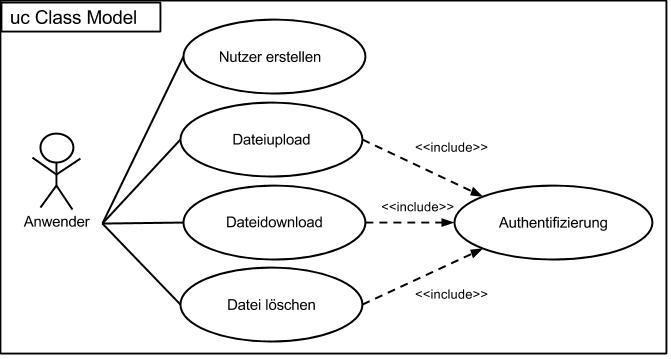
\includegraphics[width=0.7\linewidth]{UseCase.jpg}
	 \captionof{figure}{\small Anwendungsfalldiagramm}
\end{minipage}
\vspace{1em}

\textbf{AF-001 Authentifizierung:}
\begin{table}[!h]
	\centering
	\begin{tabular}{|l|l|}
		\hline
		Nummer & AF-001\\
		\hline
		Name & Authentifizierung\\
		\hline
		Akteure & Anwender\\
		\hline
		Auslöser & Anwender möchte sich anmelden\\
		\hline
		Vorbedingung & Programm zeigt den Login-Dialog, Anwender ist im \\ &  Cloud-System registriert und zum Zugriff berechtigt\\
		\hline
		Nachbedingung/Ziel & Erfolgreiche Anmeldung am Cloud-System \\
		\hline
		Nachbedingung im Sonderfall & Zugriff verweigtert\\ & Erneute Aufforderung zur Anmeldung\\
		\hline
		Normalablauf & 1. Anwender strartet Programm \\ & 2. Anwender gibt Benutzername ein \\ & 3. Anwender gibt Passwort ein \\ & 4. Zugangsdaten werden überprüft \\ & 5. 				Dateiübersicht wird angezeigt \\
		\hline
		Sonderfälle & 2a. Anwender gibt falschen oder keinen \\ & Benutzernamen ein \\ & 3a. Anwender gibt falsches oder kein Passwort ein \\ & 4a. Erneutes Laden der Loginmaske\\
		\hline
	\end{tabular}
	\caption{AF-001 Authentifizierung}
	\label{tab:AF-001 Authentifizierung}
\end{table}
\pagebreak

\textbf{AF-002 Dateiupload:}
\begin{table}[!h]
	\centering
	\begin{tabular}{|l|l|}
		\hline
		Nummer & AF-002\\
		\hline
		Name & Dateiupload\\
		\hline
		Akteure & Anwender\\
		\hline
		Auslöser & Anwender möchte eine Datei in der Cloud ablegen\\
		\hline
		Vorbedingung & Anwender hat sich erfolgreich authentifiziert \\ & Dateiübersicht wird angezeigt\\
		\hline
		Nachbedingung/Ziel & Datei wurde verschlüsselt in der Cloud abgelegt \\
		\hline
		Nachbedingung im Sonderfall & Datei kann nicht abgelegt werden\\
		\hline
		Normalablauf & 1. Anwender wählt das Menü ''File'' aus \\ & 2. Anwender wählt im Untermenü ''Select'' \\ & 3. Anwender bewegt sich durch das eigene Dateisystem \\ & zum 				Speicherpfad der hochzuladenden Datei \\ & 4. Anwender initialisiert den Dateiupload durch \\ &  Doppelklick der linken Maustaste oder Auswählen \\ & der Datei und Bestätigung                  mit ''Öffnen'' \\  & 5. Datei wird verschlüsselt \\ & 6. Datei wird hochgeladen \\
		\hline
		Sonderfälle & 5a. Datei wird nicht verschlüsselt \\ & 6a. Datei kann nicht hochgeladen werden\\
		\hline
	\end{tabular}
	\caption{AF-002 Dateiupload}
	\label{tab:AF-002 Dateiupload}
\end{table}
\pagebreak

\textbf{AF-003 Dateidownload:}
\begin{table}[!h]
	\centering
	\begin{tabular}{|l|l|}
		\hline
		Nummer & AF-003\\
		\hline
		Name & Dateidownload\\
		\hline
		Akteure & Anwender\\
		\hline
		Auslöser & Anwender möchte eine Datei aus der Cloud \\ & herunterladen\\
		\hline
		Vorbedingung & Anwender hat sich erfolgreich authentifiziert \\ & Dateiübersicht wird angezeigt\\
		\hline
		Nachbedingung/Ziel & Datei wurde aus der Cloud heruntergeladen \\ & und entschlüsselt \\
		\hline
		Nachbedingung im Sonderfall & Datei kann nicht heruntergeladen werden \\ & Datei wird nicht entschlüsselt\\
		\hline
		Normalablauf & 1. Anwender wählt in der Dateiübersicht die \\ & entsprechende Datei aus \\ & 2. Anwender wählt das Menü ''File'' aus \\ & 3. Anwender wählt im Untermenü ''Download'' \\ & 4. Anwender bewegt sich durch das eigene Dateisystem \\ & zum Speicherpfad der zu herunterladenden Datei \\ & 5. Anwender initialisiert durch ''Speichern'' \\ & den Dateidownload \\  & 6. Datei wird heruntergeladen \\ & 7. Datei wird entschlüsselt \\
		\hline
		Sonderfälle & 6a. Datei kann nicht heruntergeladen werden \\ & 7a. Datei wird nicht entschlüsselt\\
		\hline
	\end{tabular}
	\caption{AF-003 Dateidownload}
	\label{tab:AF-003 Dateidownload}
\end{table}

\textbf{AF-004 Datei l\"oschen:}
\begin{table}[!h]
	\centering
	\begin{tabular}{|l|l|}
		\hline
		Nummer & AF-004\\
		\hline
		Name & Datei löschen\\
		\hline
		Akteure & Anwender\\
		\hline
		Auslöser & Anwender möchte eine Datei aus der Cloud löschen\\
		\hline
		Vorbedingung & Anwender hat sich erfolgreich authentifiziert \\ & Dateiübersicht wird angezeigt\\
		\hline
		Nachbedingung/Ziel & Datei wurde aus der Cloud gelöscht \\
		\hline
		Nachbedingung im Sonderfall & Datei kann nicht gelöscht werden \\
		\hline
		Normalablauf & X\\
		\hline
		Sonderfälle & X \\
		\hline
	\end{tabular}
	\caption{AF-004 Datei löschen}
	\label{tab:AF-004 Datei loeschen}
\end{table}
\pagebreak

\textbf{Begriffslexikon:}

\begin{compactitem}
\item Anwender:\\
Die Rechte und Möglichkeiten des Anwenders begrenzen sich auf das Ablegen lokaler und das Herunterladen von Daten innerhalb der Cloud, sofern diese vorher beim Anbieter vergeben wurden.
\item Authentifizierung:\\
Der Login erfordert den Benutzernamen sowie das zugehörige Passwort.
\item Datei:\\
Die hochzuladende Datei kann in jedem beliebigen Dateiformat vorliegen.
\item Dateiübersicht:\\
Die Dateiübersicht gibt tabellarisch die in der Cloud abgelegten Dateien wieder. Dies beinhaltet den kryptischen Dateinamen, den originalen Dateinamen, den Zeitstempel des Ablegens sowie die Dateigröße.
\item GUI:\\
GUI (engl. Graphical User Interface) ist eine grafische Benutzeroberfläche, die dem Anwender die Interaktion mit dem System vereinfacht.
\end{compactitem}

\subsection{Installationsanleitung}
Detaillierte Beschreibung zum Einsatz auf "Fremdsystemen"
\pagebreak
\section{Binarys}
\end{appendix}

\end{document}
